	\chapter{Solving Linear System}
	In MACM 316, we will only use direct method, that is to find exact solutions in finite steps(up to round-off error).
	
	In matlab, we can use backslah "\textbackslash" to implements gaussian elimination. However, to be careful, this "\textbackslash" method in matlab is optimized for robustness but not efficiency.	
	
	\section{Count flops}
	Count flops(floating point operations) is a very useful technique to predict the fashion of computational time growth (exponential, polynomial, etc) when the size of data grows.
	
	
	The basic flops are $+,-,\times$ and $\div$. Each of the operation count as 1 flop.
	
	
	\begin{ex}
		Let $A$ be a $m\times n$ matrix, $B$ be a $n\times p$ matrix, and $x$ be a $n\times 1$ vector. Calculate the flops done in $Ax$. \\
		Since each element in $Ax$ can written as 
		\[(Ax)_i = \sum_{j=1}^n A_{ij}x_j \; \forall i=1,2,...,m\]
		so there are $(n)+(n-1) = 2n-1$ flops(n multiplications and n-1 additions) for each row of $(Ax)_i$. Since there are m rows in $Ax$, so the toatal flops is $(2n-1)m$.\\
	\end{ex}
	
	\begin{ex}
		Calculate the flops done in $AB$.\\
		Since each element in $AB$ can be written as
		\[(Ab)_{ij} = \sum_{k=1}^n A_{ik}B_{kj} \forall i=1,...,m ; j=1,...,p\]
		and there are $mp$ elements in $AB$, so the total flops is $mp(2n-1)$. \\
	\end{ex}

	\begin{ex}
		Compare the flops done in $(AB)x$ and $A(Bx)$ if $A$, $B$ is now $n\times n$, and x is still $n\times 1$.\\
		For $(AB)x$, the total flops is $n^2(2n-1) + n(2n-1)$. As for $A(Bx)$, the total flops is $n(2n-1) + n(2n-1)$. It is easy to see that although $(AB)x$ = $A(Bx)$, but $(AB)x$ does more flops than $A(Bx)$ does.
	\end{ex}	


	\section{Gaussian Elimination}
	
	\begin{ex}
		To solve the linear system
		\[ \begin{cases}
		x_1 + 5x_2 &= 7\\
		-2x_1 - 7x_2 &= -5
		\end{cases} \]
		we use Gaussian Elimination
		\[ \begin{bmatrix}
		1 & 5 &\vert 7\\
		-2 & -7 &\vert -5\\
		\end{bmatrix} 
		\Rightarrow
		\begin{bmatrix}
		1 &5 &\vert 7\\
		0 &1 &\vert 3
		\end{bmatrix}
		\]
		After elimination, we then use back substitution,
		\[ \begin{cases}
		&x_2 = \frac{3}{1} = 3\\
		&x_1 = \frac{7 - 5x_2}{1} = -8
		\end{cases} \]
	\end{ex}
	
	\begin{ex}
		Use GE to solve the linear system
		\[ \begin{cases}
		2x_2 + x_3 &= -8\\
		x_1 - 2x_2 - 3x_3 &= 0\\
		-x_1 + x_2 + 2x_3 &= 3
		\end{cases} \]
		\begin{solution}
			\[ \begin{bmatrix}
			0 &2 &1 &\vert-8\\
			1 &-2 &-3 &\vert0\\
			-1 &1 &2 &\vert3
			\end{bmatrix}
			\Rightarrow
			\begin{bmatrix}
			1 &-2& -3 &\vert0\\
			0 &2 &1 &\vert-8\\
			-1& 1& 2&\vert3\\
			\end{bmatrix}
			\]
			\[
			\Rightarrow
			\begin{bmatrix}
			1 &-2& -3 &\vert& 0\\
			0 &2 &1   &\vert&-8\\
			0 &-1& -1 &\vert& 3
			\end{bmatrix}
			\Rightarrow		
			\begin{bmatrix}
			1 &-2& -3   &\vert& 0\\
			0 & 2&  1   &\vert&-8\\
			0 & 0& -0.5 &\vert&-1
			\end{bmatrix}	
			\]
			
			Now we use the back substitution,
			\[\begin{cases}
			&x_3 = \frac{-1}{-0.5} = 2\\
			&x_2 = \frac{-8-x_3}{2} = -5\\
			&x_1 = \frac{0 + 2x_2 + 3x_3}{1} = -4 
			\end{cases}\]
		\end{solution}
	\end{ex}
	
	\subsection{flops counting}
	GE(Gaussian Elimination) consists of two parts, elimination and back substitution.
	
	Back substitution:
	For $i=n$:
	\[\frac{b_n}{a_{nn}} \Rightarrow 1\;\text{division} \Rightarrow 1\;\text{flop}\] 
	
	For $1\leq i \leq n-1$:
	\begin{enumerate}
	\item \[\sum_{j=i+1}^n a_{ij}x_j \Rightarrow n-i-1\;\text{addition},n-i\;\text{multiplication} \]
	
	\item \[  b_i-\sum_{j=i+1}^n a_{ij}x_j  \Rightarrow 1\;\text{subtration}\]
	
	\item \[ \frac{b_i-\sum_{j=i+1}^n a_{ij}x_j}{a_{ii}} \Rightarrow 1\;\text{division}\]
	\end{enumerate}
	Totally $(n-i-1)+(n-i)+1+1=2(n-i)+1$ flops.\\
	Therefore, total flops in back substitution can be calculated:
	\begin{align*}
	1 + \sum_{i=1}^{n-1} [2(n-i)+1] &= 2(n-n) +1 + \sum_{i=1}^{n-1} [2(n-i)+1] \\
	&=\sum_{i=1}^n [2(n-i)+1]\\
	&= \sum_{i=1}^n (2n+1) - \sum_{i=1}^n 2i\\ 
	&= n(2n+1) -2\frac{n(1+n)}{2} \\
	&= n^2
	\end{align*}
	Therefor back subtitution requires exactly $n^2$ flops. And we can also show that elimination requires $\frac{2}{3}n^3 + O(n^2)$ flops. Therefore, Gaussian Elimination requires totally $\frac{2}{3}n^3 + O(n^2)$ flops to finish the calculation.
	
	\subsection*{Partial Pivoting}
	GE is not stable. Here is an example:
	\begin{ex}
	\[ \begin{cases}
		&0.0030000x_1 + 59.14x_2 = 59.17\\
		&5.291x_1 - 6.130x_2 = 46.78
	\end{cases} \]

	The EXACT solution of this system is $x_1 = 10.000000$ and $x_2 = 1.000000$. However, the solution calculated through GE is $x_1 = -10.00$ and $x_2 = 1.001$ if 4 digits rounding applied. Here is the calculation:
	
	\[
	\begin{bmatrix}
	0.003000 & 59.14 &| &59.17\\
	5.291    & -6.130 &| &46.78
	\end{bmatrix}  
	\Rightarrow
	\begin{bmatrix}
	0.003000 & 59.14 &| &59.17\\
	     0   & -104300 &| & -104400
	\end{bmatrix}  
	\]
	
	we have that
	\begin{align*}
	&x_2 = -104400/ -104300 \approx 1.001  \text{(four digits rounding)}\\
	&x_1 = (59.17-59.14\cdot1.001)/0.003000 \approx -10.00  \text{(not right at all!)}
	\end{align*}
	\end{ex}
	
	To fix the problem, always put the number with larger absolute value to the operating row. This is so called partial pivoting, and it improves the stability of calculation.
	
	\begin{ex}
		Do partial pivoting to the system as we doing elimination
		\[\begin{bmatrix}
		0.003000 & 59.14 &| &59.17\\
		5.291    & -6.130 &| &46.78
		\end{bmatrix}
		\]
		Since $|0.003000| < |5.291|$, so we interchange row 1 and row 2, $E_1 \leftrightarrow E_2$.
		\[
		\underset{E_1 \leftrightarrow E_2}{\Rightarrow}
		\begin{bmatrix}
		5.291    & -6.130 &| &46.78\\
		0.003000 & 59.14 &| &59.17
		\end{bmatrix}\]
		
		\[\Rightarrow
		\begin{bmatrix}
		5.291    & -6.130 &| &46.78\\
		0    & 59.10533926 &| & 59.14347571
		\end{bmatrix}\]
		\[
		\Rightarrow
		\begin{bmatrix}
		7.683\\
		1.000
		\end{bmatrix}
		\]
	\end{ex}
	
	
	We see that the answer improved alot.
	
	
	\begin{summary}
		When doing Gaussian Elimination, remember that
		\begin{enumerate}
			\item Always do partial pivoting.
			\item Partial pivoting increases the robustness of the computation to round-off error.
			\item It ensures the division is always $\frac{small}{big}$, so the amplification of round-off error won't happen.
		\end{enumerate}
	\end{summary}
	
	
	\subsection*{Scaled Partial Pivoting}
	Partial pivoting works for most of the time, but still, there are situations it fails. 
	\begin{ex}
		Try partial pivoting for the following linear system(again using 4-digit rounding), it will fail!
		\[ \begin{cases}
		&30.00x_1 + 591400x_2 = 591700\\
		&5.291x_1 - 6.130x_2 = 46.78
		\end{cases} \]
		We see that this system is the system we've shown in Example 5. It's just the first row being multiply by a factor of $10^4$. So the EXACT solution is still $x_1 = 10$ and $x_2 = 1$.
		
		We do with partial pivoting, since $\max{30.00, 5.291} = 30.00$, so no need to do row interchanges (while in Example 6, we did row interchanges!). Then we do elimination,
		\[ \begin{bmatrix}
		30.00 & 591400 & \vert &591700\\
		0     &-104300 & \vert & -104400

		\end{bmatrix} \]
		using back substitution, we get 
		\begin{align*}
		x_2 &= \frac{-104400}{-104300} = 1.001\\
		x_1 &= \frac{591700 - 591400\times1.001}{30.00} = -10.00
		\end{align*}
		Same error occurs!!!
	\end{ex}

	It turns out the thing that really matters is the relative magnitude instead of the absolute magnitude(though that works for most of time). So scaled pivoting comes into play. 
	
	
	\begin{ex}
		Solve the linear system using scaled partial pivoting
		\[ \begin{cases}
		2.11x_1 - 4.21x_2 + 0.921x_3 &= 2.01\\
		4.01x_1 + 10.2x_2 -  1.12x_3 &= -3.09\\
		1.09x_1 + 0.987x_2 +0.832x_3 &= 4.21.
		\end{cases} \]
	\end{ex}
	\begin{solution}
		The augmented matrix
		\[ \begin{bmatrix}
		2.11 & -4.21 & 0.921 & \vert & 2.01\\
		4.01 & 10.2  & -1.12 & \vert & -3.09\\
		1.09 & 0.987 & 0.832 & \vert & 4.21
		\end{bmatrix} \]
		
		We have s1 = 4.21, s2 = 10.2, and s3 = 1.09. So,
		\[ \frac{|a_{11}|}{s_1} = \frac{2.11}{4.21} = 0.501,\;\; 
		\frac{|a_{21}|}{s_2} = \frac{4.01}{10.2} = 0.393,\;\;
		\frac{|a_{31}|}{s_3} = \frac{1.09}{1.09} = 1 \]
		
		Since $|a_{31}|/s_3$ is largest, we perform $E_1 \leftrightarrow E_3$ to obtain
		\[ \begin{bmatrix}
		1.09 &0.987& 0.832& \vert& 4.21\\
		4.01 &10.2 &-1.12 &\vert &-3.09\\
		2.11 &4.21 & 0.921& \vert& 2.01
		\end{bmatrix} \]
		Then perform first two elimination,
		\[ \begin{bmatrix}
		1.09 &0.987 &0.832 &\vert &4.21\\
		0    &6.57  &-4.18 &\vert &-18.6\\
		0    &-6.12 &-0.689& \vert& -6.16
		\end{bmatrix} \]
		
		Now we do the scaled pivoting again, since 
		\[ \frac{|a_{22}|}{s_2} = \frac{6.57}{10.2} = 0.644,\;\;
		\frac{|a_{32}|}{s_3} = \frac{6.12}{4.21} = 1.45 \]
		
		Since $|a_{32}|/s_3$ is larger, so we swap rows $E_2 \leftrightarrow E_3$.
		\[ \begin{bmatrix}
		1.09 &0.987 &0.832 &\vert &4.21\\
		0    &-6.12 &-0.689& \vert& -6.16\\
		0    &6.57  &-4.18 &\vert &-18.6
		\end{bmatrix} \]
		Again, we do elimination,
		\[ \begin{bmatrix}
		1.09 &0.987 &0.832 &\vert &4.21\\
		0    &-6.12 &-0.689& \vert& -6.16\\
		0    &0     &-4.92 &\vert &-25.2
		\end{bmatrix} \]
		Finally, backward substitution gives the solution $x_1 = -0.431$, $x_2 = 0.430$, and $x_3 = 5.12$.
	\end{solution}
	
	\begin{summary}
		Here is the summary for scaled pivoting.
		\begin{enumerate}
			\item Although partial pivoting works most of the time, it may also fail.
			\item Scaled partial pivoting is more robust than just partial pivoting.
			\item The efficiency of scaled pivoting is not as good as partial pivoting.
			\item The fundamental reason that causes the problem is not ABSOLUTE magnitude of the pivoting, but the RELATIVE magnitude of the pivoting.
			\item The scale factor only compute once at the start of the calculation.
		\end{enumerate}
	\end{summary}
	
	\subsection*{Complete Pivoting}
	Choose $a_{mp}^{(k-1)}$ as the pivot for step k, where 
	\[ |a_{mp}^{(k-1)}| = \max_{\substack{k\leq i\leq n,\\ k\leq j\leq n}} |a_{ij}^{(k-1)}| \]
	This is the most robust way to solve a linear system.
	  
	\begin{ex}
		Solve the linear system using complete pivoting
		\begin{align*}
		0.0030000x_1 + 59.14x_2 = 59.17\\
		5.291x_1 - 6.130x_2 = 46.78
		\end{align*}
	\end{ex}
	\begin{solution}
		The augmented matrix is
		\[
		\begin{bmatrix}
		0.003000 & 59.14 &| &59.17\\
		5.291    & -6.130 &| &46.78
		\end{bmatrix}  
		\]
		The first pivot $a_{11}^{(1)} = \max\{0.003000, 59.14, 5.291, 6.130\} = 59.14$, thus we perform column exchanges $C_1\leftrightarrow C_2$. Be careful that the order of variables has been changed($x_1\leftrightarrow x_2$).
		\[ \begin{bmatrix}
		59.14 & 0.003000 &| &59.17\\
		-6.130 & 5.291 &| &46.78
		\end{bmatrix} \]
		We then do elimination
		\[ \begin{bmatrix}
		59.14 & 0.003000 &| &59.17\\
		0 & 5.291 &| &52.91
		\end{bmatrix} \]
		
		using back substitution
		\begin{align*}
		x_1 &= \frac{52.91}{5.291} = 10.00\\
		x_2 &= \frac{59.17 - 0.003000x_1}{59.14} = 1.000
		\end{align*}
		
		We have the EXACT solution when we perform complete pivoting.
	\end{solution}
	\begin{summary}
		Here is the performance of each algorithms.
		\item Efficiency: GE $>$ partial pivoting $>$ scaled pivoting $>$ complete pivoting.
		\item Robustness: GE $<$ partial pivoting $<$ scaled pivoting $<$ complete pivoting.
		
		And the flops of each algorithm:
		\begin{enumerate}
			\item 
			GE: $\frac{2}{3}n^3 + O(n^2)$
			\item 
			Partial pivoting: not much change.
			\item 
			Scaled pivoting: not much change.
			\item 
			Complete pivoting: additional $\frac{n(n-1)(2n+5)}{6}$ comparisons.
		\end{enumerate}
	\end{summary}
	
	
	\section{Condition number}
	
	\begin{definition}
		The condition number $\kappa$ of an invertible matrix $A$ is 	
		\[\kappa(A) = \sqrt{\frac{\lambda_{max}(A^\dagger A)}{\lambda_{min}(A^\dagger A)}}
		= \frac{\sigma_{max}(A)}{\sigma_{min}(A)}
		= \left\| A \right\|_2 \left\| A^{-1} \right\|_2\]
	Where $\lambda_{max}(A^\dagger A) (or\;\lambda_{min}(A^\dagger A))$ means the maximum(or minimum) eigenvalue of $A^\dagger A$; $\sigma_{max}(A) (or\;\sigma_{min}(A))$ means the maximum(or minimum) singular value of the matrix $A$; and lastly, $\left\| A \right\|_2$ means the matrix norm of $A$.
	
	If $\kappa(A)\approx 1$, then A is well conditioned, $\kappa(A) >> 1$ means A is ill conditioned. 
	\end{definition}
	
	\begin{thm}
		When calculating the solution of a linear system, the error
		
		\[err = \underset{{i=1,..,N}}{\max} |x_i - \hat{x}_i| \approx \kappa(A)\cdot\epsilon \]
		
		Where $\epsilon$ is the machine epsilon.
	\end{thm}

	So the condition number determines the robustness.
	Worth to mention, DFT matrix is well conditioned(actually perfect) since $\kappa(DFT) = 1$ and Hilber matrix is ill conditioned since $\kappa(Hilber matrix) \approx 34^N$ (where N is the size of Hilber matrix).
	
	\begin{summary}
		Here are some things that we need to know: 
		\begin{enumerate}
			\item MATLAB has built-in warinings for ill-conditioned matrix. rcond() command in MATLAB computes $1/\kappa$.
			
			\item When dealing ill conditioned matrix we always get bad solutions($err = \kappa(A)\cdot\epsilon$) regarless which algorithm we use, this is not a failure of numerical algorithms.
			
			\item $\kappa(A)$ is a intrinsic property of the linear system, regardless of the algorithm.
		\end{enumerate}     
	\end{summary}
	 
	
	
	
	\section{LU decomposition}
	Suppose we want to solve the linear system $ A\vec{x} = \vec{y}$
	For any row operations: $E_i = \lambda E_j + E_i$, we define elmentary matrix as:
	\[ E_{ij} = \left \{\begin{matrix}
	\text{diagonal} = 1\\
	a_{ij} = \lambda\\
	\text{others} = 0
	\end{matrix} \right. 
	\;\; \;
	E_{ij}^{-1} =\left\{  \begin{matrix}
	\text{diagonal} = 1\\
	a_{ij} = -\lambda\\
	\text{others} = 0
	\end{matrix} \right.
	\]
	
	Notice that $E_{ij}^{-1}$ is the inverse matrix of $E_{ij}$, means that it's doing a reverse row operation. And it is worth to mention that according to the definition of elementary matrix(and their inverse), they are commutative.
	
	When doing GE, we get a upper triangular matrix after the elimintion process, denoted as U. And record down the row operations we did when doing eliminations as $E_{ij}$. Then the matrix A can be decomposed to

	\[ A =  LU \;\; (\text{where}\; L =\prod_{i=1} E_{jk}^{-1\,(i)})\]
	
	and L is a lower triangular matrix.
	
	E.x. Let $A = \begin{bmatrix} 1 & 3 & 2 \\ 2 & 7 & 3 \\ 0 & 2 & 2 \end{bmatrix}$.  Find its LU decomposition. 
		\[ \begin{bmatrix} 1 & 3 & 2 \\ 2 & 7 & 3 \\ 0 & 2 & 2 \end{bmatrix} 
		\underset{E_2 = E_2 -2E_1}{\Rightarrow} \begin{bmatrix} 1 & 3 & 2 \\ 0 & 1 & -1 \\ 0 & 2 & 2 \end{bmatrix}
		\underset{E_3 = E_3 -2E_2}{\Rightarrow} \begin{bmatrix} 1 & 3 & 2 \\ 0 & 1 & -1 \\ 0 & 0 & 4 \end{bmatrix}\]
	
	So $U = \begin{bmatrix} 1 & 3 & 2 \\ 0 & 1 & -1 \\ 0 & 0 & 4 \end{bmatrix}$. And according to the row operations we did, the matrix L should be:
	
	\[ L = \begin{bmatrix} 1 & 0 & 0 \\ 2 & 1 & 0 \\ 0 & 0 & 1\end{bmatrix} 
	\begin{bmatrix} 1 & 0 & 0 \\ 0 & 1 & 0 \\ 0 & 2 & 1\end{bmatrix} 
	= \begin{bmatrix} 1 & 0 & 0 \\ 2 & 1 & 0 \\ 0 & 2 & 1\end{bmatrix}\]
	
	Some important things: (Let's denot $U\vec{x}$ as $\vec{a}$.)
	\begin{enumerate}
		\item To factorize $A$ to $L$ and $U$, it takes $\frac{2}{3}n^3$.
		\item  Doing forward substitution to solve $\vec{a}$ from $L(U\vec{x}) = \vec{y}$ takes $n^2$ flops.
		\item Doing backward substitution to solve $\vec{x}$ from  $U\vec{x} = \vec{a}$ takes $n^2$ flops.
		\item To solve a linear system $A\vec{x} = \vec{y}$ by LU decomposition takes $\frac{2}{3}n^3 + 2n^2$ flops.
	\end{enumerate}
	
	Applications of LU decomposition:
	\begin{enumerate}
		\item The single calculation is slower than GE, but it is faster when we are solving multiple equations $A\vec{x}^{(i)} = \vec{y}^{(i)}, \; i=1,2,...,k$ with same matrix $A$. Since solving k similar equations takes $\frac{2}{3}n^3 + n^2 k$ for LU decomposition but $\frac{2}{3}n^3 k$ for GE. Moreover, LU method is generally more robust than GE.
		\item It is convienient to computing determinant of an $n\times n$ matrix $A$, since $\det(A) = \det(L)\det(U) = \prod_{i=1}^{n} L_{ii}U_{ii}$, where $L_{ii}$ and $U_{ii}$ are main diagonal elements. 
	\end{enumerate}
	
	\subsection{LU decomposition with pivoting}
	Suppose there exists a permutation matrix $P$ such that $PA\vec{x} = P\vec{y}$ can be solved without doing row interchange. Then we can factor $PA = LU$, and now $A = P^{-1}LU$. This is called LU decomposition of A with pivoting.
	
	Note that $P^{-1} = P^{T}$, and $P$ (or $P^{-1}$) can be stored easily, only needs to store n values if $P$ is $n\times n$.
	
	To get $P$, just simply interchange the rows of an identity matrix with the same size.
	

	\begin{ex}
		Find $P$ if $E_1 \leftrightarrow E_2$, $E_2 \leftrightarrow E_4$.
		\[ \{1,2,3,4\} \Rightarrow \{2,1,3,4\} \Rightarrow \{2,4,3,1\} \Rightarrow P = \begin{bmatrix}
		0 & 1 & 0 & 0 \\  0 & 0 & 0 & 1 \\ 0 & 0 & 1 & 0 \\ 1 & 0 & 0 & 0 \\
		\end{bmatrix} \]
	\end{ex}
	
	
	Algorithm to find $P$, $L$, $U$ for a matrix $A$:
	\begin{enumerate}
		\item Do GE with pivoting to A, then we'll get U.\\
		\item Observe what row interchange we've done, then find P.\\
		\item Apply GE to the matrix $PA$ to find L by recording the row operations (but no row interchange this time).
	\end{enumerate}
	
	In MATLAB, just simply use the command [L U] = lu(A) or [L U P] = lu(A) to get all three matrices. But be very careful that in the first command [L U] = lu(A), L maynot be lower triangular since this $L$ is actually $PL$.


	\section{Special Matrix}
	\subsection{Diagonally Dominant Matrices}
	
	\begin{definition}
		A $n\times n$ matrix is said to be diagonally dominant if
		\[ |a_{ii}| \geq \sum_{\substack{j=1,\\ j\neq i}}^n|a_{ij}|,\;\; \forall i = 1,2,3,...,n. \] 
		A diagonally dominant matrix is said to be strictly diagonally dominant when the inequality is strict for each n, that is, when
		\[  |a_{ii}| > \sum_{\substack{j=1,\\ j\neq i}}^n|a_{ij}|,\;\; \forall i = 1,2,3,...,n. \]
	\end{definition}

	\begin{ex}
		\[ A = \begin{bmatrix}
		7 & 2 & 0 \\
		3 & 5 & -1\\ 
		0 & 5 & -6
		\end{bmatrix},\;\;\;
		B =\begin{bmatrix}
		6 & 4  & -3\\ 
		4 & -2 & 0 \\
		-3 & 0 & 1 
		\end{bmatrix}
		 \]
		 
		 $A$ is strictly diagonally dominant since 
		 \[|7| > |2|+|0|,\;\; |5| > |3|+|-1|,\;\; and\;\; |-6| > |0|+|5|. \]  
		 while $B$ is not diagonally dominant because in its first row, we have $|6| < |4|+|-3|= 7$.
		 
		 It is worth to mention that: $M$ is diagonally dominant $\not\Rightarrow$ $M^T$ is diagonally dominant. We can see that in this  example, $A^T$ is not diagonally dominant while $A$ is.
	\end{ex}

	\begin{thm}
		A strictly diagonally dominant matrix A is nonsingular. Moreover, in this case, Gaussian elimination can be performed on any linear system of the form $A\mathbf{x} = \mathbf{b}$ to obtain its unique solution without row or column interchanges, and the computations will be stable with respect to the growth of round-off errors.
	\end{thm}
	
	
	\subsection{Others}
	\begin{enumerate}
		\item [I.] Symmetric matrix: $A = A^T$.
		\item [II.] Positive definite matrix: $\vec{x}^T A \vec{x} > 0, \; \forall \vec{x} \neq \vec{0}$.
		\item [III.] A symmetric, positive definite matrix, A, has a Cholesky fcatorization $A = LL^T$. Where L is lower triangular with positive diagonal entries.
	
	
	Remark:
	\begin{enumerate}
		\item The Cholesky factorization is $O(\frac{n^3}{3})$. Half of the time of LU decomposition.\\
		\item No pivoting is needed. Positive definite property ensures that it is robust to round-off error.
	\end{enumerate} 
	
	\item [IV.] Tridiagonal matrix: the entries $a_{ij} = 0$ if $|i-j|>1$.\\
	An example: 
	\[ A = \begin{bmatrix} 
	1 & 2 & 0 & 0\\  
	-2 & 3 & 2 & 0 \\
	0 & 1 & 5 & -2\\
	0 & 0 & 6 & 4 
	\end{bmatrix} \] 
	\item [V.] Tridiagonal matrix can be very efficiently LU decomposed, only takes $O(8n)$ flops when n is large:
	
	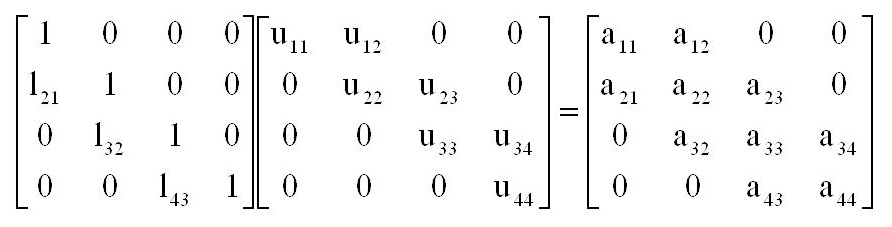
\includegraphics[width=10cm]{img/tridiagonal_matrix}\\
	\item [VI.] Sparse matrix: Matrices whose entries are mainly zeros.
	
	 
	\end{enumerate}
	
	